% implementation structures O(1), Vertex, Triangle, Observables

\newcommand{\tup}{\bigtriangleup}
\newcommand{\tdown}{\raisebox{\depth}{$\bigtriangledown$}}

% Store the geometry
% Naïve solution: use slice structure to store a sequence of up-down
% Performing moves meaning moving triangles, meaning O(N) complexity
% Solution: store list with connectivities

\begin{frame}
    \frametitle{Implementation}
    We need some representation of the triangulation
    \begin{itemize}
        \item Naïve solution: store a sequence of $\tup$ and \tdown \\
        \quad $[[\tup, \tdown, \tdown],
        [\tdown, \tup],
        [\tdown, \tup, \tup, \tdown, \tup],
        \cdots]$ \\
        \quad $\hookrightarrow$ Performing moves has $\order{N}$ complexity
        \item Alternative: store the adjacency or connectivity % similar to lecture DT
    \end{itemize}
    % If possible add image of adjacency
    And we require an initial state: \emph{flat geometry}
\end{frame}

% Distances are of intrest so natural to look at connectivity of vertices
% Computationally simplier is to look at connectivity of triangles
% Finally: store an ordered list where every element represents a triangle, which stores the triangle indices it is connected to, and it's type (up-down)
% In this way both moves can be done in O(1), the 4-4 move without rejection and the 2-2 flip with rejection rate of approximately 50%
\begin{frame}
    \frametitle{Vertices or Triangles}

    One can store the adjacency of the vertices or triangles
    \begin{itemize}
        \item Vertices more natural % As we're interseting in distances which we measure as graph distance between vertices
        \item Vertices have \emph{variable amount} of neighbours
        \item Triangles always have \emph{three} neighbours
        \item Triangles have two types ($\tup$ and \tdown)
    \end{itemize}
    Finally chose triangle-based implementation
    \begin{itemize}
        \item Store ordered list of triangles: $[(\tup, 7, 21, 1), (\tdown, 0, 12, 4), \cdots]$
        \item Moves performed by updating adjacency
    \end{itemize}
\end{frame}


% To be able to analyse the behaviour of the model, meaningful observables need to be found
% These observables cannot depend on the labels, and have no 'positional' information, as the system is fully periodic
% Interesting to look at the behaviour of the spatial size of the universe: here simply counting the number of space-like links on the boundaries of the timeslices; this already gets rid of the spatial dependence.
% To get rid of the time dependence we can perform an average (this is trivially L as we keep N constant), look at the standard deviation, look at the autocorrelation of spatial size over time (using periodic boundaries, to be able to do so T need to be sufficiently large).

\begin{frame}
    \frametitle{Observables}

    
    \begin{itemize}
        \item Difficult to find meaningful observables
        \item Cannot depend on labeling $\rightarrow$ 'sum' over geometry
        \item Consider spatial size of timeslices (link length)
        \item Length profile: mean, \emph{standard deviation}, \emph{autocorrelation}
    \end{itemize}
    \begin{figure}
       \centering
       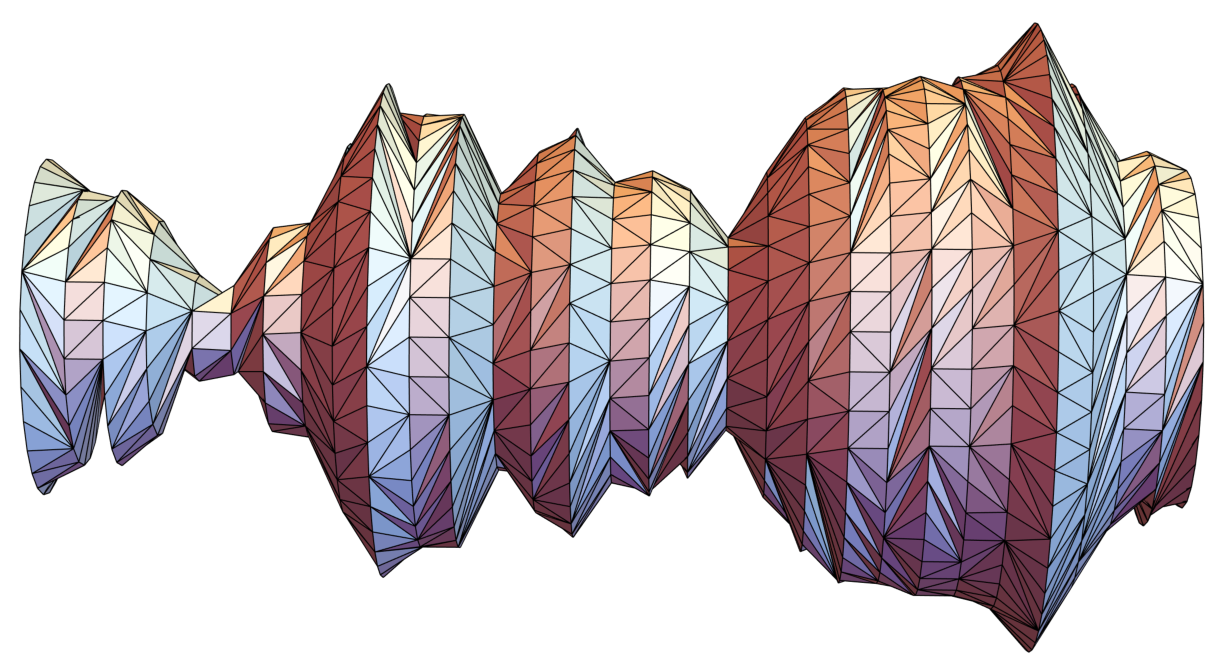
\includegraphics[width=0.6\linewidth]{img/triangulation.pdf}    
    \end{figure}
\end{frame}

% To get the length profile out of the adjacency data we 'walk' through the triangulation along slices first (recording the amount of up-triangles) until going around fully; then advance up via a down triangle and repeat; until the original slice is again reached.

\begin{frame}
    \frametitle{Length profile}

    Obtaining the length profile is not entirely trivial:
    \begin{itemize}
        \item 'Walk' through the triangulation
        \item Record number of $\tup$ (equivalent to vertex distance)
        \item Move to next timeslice (using \tdown)
        \item Complexity of $\order{N}$ \\[3mm]% Note that this would be simpler in naive list
        \item Visualisation by similar mesh creation
        % For visualisation of the triangulation we do something similar but in stead of counting the number of up-triangles, we label the vertices and record to which triangle they belong; in the end yielding a list of triangles each with three labels to vertices
        % Then we choose an embedding, one that obeys the slice behaviour, meaning the coordinates of the vertices are chosen; from this the triangulation can be visualized. This embedding may also be 2D 
    \end{itemize}
    % TODO: possibly add image of such a walk
\end{frame}